\documentclass{article}
\usepackage[margin=1in]{geometry}
\usepackage{fancyhdr}
\usepackage{graphicx}
\usepackage{amsmath}
\usepackage{cancel}
\usepackage{caption}
\usepackage{nccmath}
\usepackage{amssymb}
\usepackage{array}
\usepackage{tikz}
\graphicspath{ {images/} }

\usepackage{tikz}
\newcommand*\circled[1]{\tikz[baseline=(char.base)]{
            \node[shape=circle,draw,inner sep=2pt] (char) {#1};}}

\pagestyle{fancy}
\lhead{BME 384}
\rhead{Pascale Walters 20566177\\
		Lee Yu Wu 20558313}

\begin{document}

\begin{center}\underline{\huge Hands-On Fluids Challenge}\end{center}

\section{Theoretical Calculation: Height of the Jet Stream}
%
The first objective of the experiment is to model the height of the jet as a function of the speed of the displacement of the piston of the syringe. This is accomplished by defining a relationship between the velocity of the fluid leaving the tip of the needle at \circled{2} and the velocity of the fluid at the highest point of the jet stream at \circled{3} through the mass balance equation and Bernoulli's Principle. These locations are illustrated in Figure \ref{fig:1}.

%
\begin{figure}[h!]
\centering
  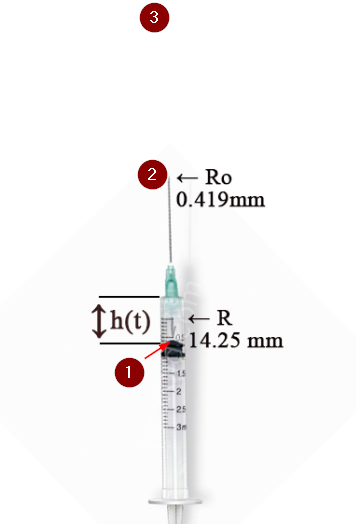
\includegraphics[width=50mm]{Syringe.png}
  \captionsetup{justification=centering}
  \caption{An illustration of the syringe. The label points are used in mass balance and Bernoulli.}
  \label{fig:1}
\end{figure}
%
From the mass balance equation,
\begin{align*}
0= \frac{\partial}{\partial{t}} \int_{cv} \rho dv + \int_{cs} \rho \bar{v} \cdot d\bar{A} \label{eq:1-1} \tag{1-1} 
\end{align*} 

The control volume consists of the entire syringe (i.e. all volumes enclosed between \circled{1} and \circled{2}). As there is fluid existing the control volume, $\frac{\partial}{\partial{t}} \int_{cv} \rho dv$ is non zero. Integrating the two terms shown in \eqref{eq:1-1} yields the following results:

\begin{align*}
\frac{\partial}{\partial{t}} \int_{cv} \rho dv = \frac{dm}{dt}
\end{align*}
\begin{align*}
\int_{cs} \rho \bar{v} \cdot d\bar{A} = \rho \bar{v_2} \pi R_o^2
\end{align*}

Substituting the individual terms into \eqref{eq:1-1} results in
\begin{align*}
\frac{dm}{dt} = - \rho \bar{v_2} \pi R_o^2
\end{align*}
\begin{align*}
\rho \pi R^2 \frac{dh}{dt} = \rho \pi \bar{v_2} R_o^2
\end{align*}
Since the jet stream is a free jet, the velocity profile can be assumed to be uniform and therefore, $\bar{v_2} = v_2$.
\begin{align*}
\frac{dh}{dt} = -(\frac{R_o}{R})^2 v_2
\end{align*}
\begin{align*}
v_2 = -\frac{dh}{dt} (\frac{R}{R_o})^2
\end{align*}

The highest point of the jet stream (i.e. \circled{3}) is related to the exist velocity at \circled{2} by Bernoulli's Principle.
\begin{align*}
\frac{P_2}{\rho} + g z_2 + \frac{\alpha v_2^2}{2} = \frac{P_3}{\rho} + g z_3 + \frac{\alpha v_3^2}{2} 
\end{align*}
Taking $z_2$ as the reference point reduces the term to zero and the velocity at the highest point is also zero.
\begin{align*}
\frac{P_2}{\rho} + g \cancelto{0}{z_2} + \frac{\alpha v_2^2}{2} = \frac{P_3}{\rho} + g z_3 + \frac{\alpha \cancelto{0}{v_3^2}}{2} \label{eq:1-2} \tag{1-2}
\end{align*}
where
\begin{align*}
P_2 = P_atm + P_c
\end{align*}
\begin{align*}
P_c = \frac{2\gamma}{d} = \frac{2\gamma}{2 R_o} = \frac{\gamma}{R_o}  \textrm{ and } \gamma = 72 \frac{mN}{m}  \textrm{ for air-water interface}
\end{align*}
and $\alpha = 2$, laminar flow, can be assumed as the diameter of the needle is small and the velocity is extremely slow (i.e. on the order of mm/s), therefore resulting in a small $N_{Re}$. Substituting \eqref{eq:1-1} back to \eqref{eq:1-2}:
\begin{align*}
z_3 = \frac{1}{g} (\frac{\gamma}{R_o \rho} + (\frac{dh}{dt})^2(\frac{R}{R_o})^4)  \label{eq:1-3} \tag{1-3}
\end{align*}
where $z_3$ is the highest point the jet stream can reach in meters.

\begin{multline*}
z_3 = \frac{1}{9.81} (\frac{72\times10^{-3}}{0.419\times10^{-3} \times 1000} + (\frac{dh}{dt})^2(\frac{14.25\times10^{-3}}{0.419\times10^{-3}})^4)\\= 0.102\times(0.172 + (\frac{dh}{dt})^2 \times1.34\times{10^6}) \textrm{ where $\frac{dh}{dt}$ varies in each experiment}
\end{multline*}

\section{Theoretical Calculation: Magnitude of Force Applied on Piston}

Mass balance on the control volume (refer to Figure \ref{fig:1} for the position of each point. In this case, \circled{1} is a point within the syringe just below the start of the needle):
\[ v_{1}A_{1} = v_{2}A_{2} \]
\[ v_{1}\pi{R}^2 = v_{2}\pi{R_{o}}^2 \]
\[ \Rightarrow v_{2} = v_{1} \left(\frac{R}{R_{o}}\right)^2 \tag{2-1} \label{eq:1} \]

Where $v_{1}$ is the velocity at which the piston is pushed and $v_{2}$ is the velocity of the jet of water as it leaves the needle tip. \\

Bernoulli between the same \circled{1} and \circled{2} :
\[ \frac{P_{1}}{\rho} + \alpha_{1}\frac{{v_{1}}^2}{2}  + gz_{1} = \frac{P_{2}}{\rho} + \alpha_{2}\frac{{v_{2}}^2}{2}  + gz_{2} + h_{f} \tag{2-2} \label{eq:2} \]

Where,
\[ P_{2} = P_{atm} + P_{capillary}  = P_{atm} + \frac{\gamma}{R_{o}} \]


Using $v_{2}$ from \eqref{eq:1} and assuming laminar flow ($\alpha_{1} = \alpha_{2} = 2$), \eqref{eq:2} becomes:
\[ \frac{P_{1}}{\rho} + {v_{1}}^2 = \frac{P_{atm} + \frac{\gamma}{R_{o}}}{\rho} + {v_{1}}^2\left(\frac{R}{R_{o}}\right)^4  + gl_{needle} + h_{f} \]

Laminar flow can be assumed because the diameter of the needle is very small and the speed of the water is relatively low.

Solving for $P_{1}$,
\[ P_{1} = P_{atm} + \frac{\gamma}{R_{o}} + \rho{v_{1}}^2\left[\left(\frac{R}{R_{o}}\right)^4  - 1 \right] + \rho gl_{needle} + \rho h_{f} \tag{2-3} \label{eq:3} \]

All values are known in this equation, except for $h_{f}$. The losses due to friction are given as:
\[ h_{f} = 4f_{needle} \frac{l_{needle}}{2R_{o}} \frac{{v_{2}}^2}{2} = 4f_{needle} \frac{l_{needle}}{2R_{o}} \frac{{v_{1}}^2}{2} \left(\frac{R}{R_{o}}\right)^2 \tag{2-4} \label{eq:4} \]

Minor losses will be neglected because they will be much smaller than the major losses, due to the ratio of the length of the needle to its diameter being very large. Since the flow was assumed to be laminar, the friction factor is:
\[ f = \frac{16}{N_{Re}} \tag{2-5} \label{eq:5} \]

Where $N_{Re}$ is the Reynolds number given by:
\[ N_{Re} = \frac{\rho v_{2} (2R_{o})}{\mu} = \frac{2 \rho v_{1} R^{2}}{\mu R_{o}} \tag{2-6} \label{eq:6} \]

Substituting \eqref{eq:6} into \eqref{eq:5}:

\[ f = \frac{8 \mu R_{o}}{\rho v_{1} R^{2}} \tag{2-7} \label{eq:7} \]

Substituting \eqref{eq:7} into \eqref{eq:4}:

\[ h_{f} = \frac{8 \mu R_{o}}{\rho v_{1} R^{2}} \frac{l_{needle}}{R_{o}} {v_{1}}^2 \left(\frac{R}{R_{o}}\right)^2 = \frac{8 \mu l_{needle} v_{1} }{\rho {R_{o}}^2} \tag{2-8} \label{eq:8} \]

Substituting \eqref{eq:8} into \eqref{eq:3}:
\[ P_{1} = P_{atm} + \frac{\gamma}{R_{o}} + \rho{v_{1}}^2\left[\left(\frac{R}{R_{o}}\right)^4  - 1 \right] + \rho gl_{needle} + \frac{8 \mu l_{needle} v_{1} }{{R_{o}}^2} \tag{2-9} \label{eq:9} \]

The forces acting on the piston are the sliding friction force $F_{s}$ and the force due to the pressure of the water in the syringe $P_{1}A_{1}$. These forces oppose the applied force on the syringe $F$. From Newton's second law,
\[ \Sigma F = ma \]

For the piston to move at a constant velocity,
\[ \Sigma F = 0 \]
\[ \therefore F = F_{s} + P_{1}A_{1} \tag{2-10} \label{eq:10} \]

Substituting \eqref{eq:9} into \eqref{eq:10},
\[ F(v_{1}) = F_{s} + \left[P_{atm} + \frac{\gamma}{R_{o}} + \rho{v_{1}}^2\left[\left(\frac{R}{R_{o}}\right)^4  - 1 \right] + \rho gl_{needle} + \frac{8 \mu l_{needle} v_{1} }{{R_{o}}^2} \right] \pi R^{2}\]

As determined experimentally, $F_{s} = 35.6 \ N$. Substituting in other known values,
\begin{multline*}
F(v_{1}) = 35.6 \ N + \\ \bigg[ 101.325 \times 10^{3} \ Pa + \frac{72 \times 10^{-3} \ N/m}{0.419 \times 10^{-3} \ m} +\left(1000 \ kg/m^3 \right) {v_{1}}^2 \left[\left(\frac{14.25 \times 10^{-3} \ m}{0.419 \times 10^{-3} \ m}\right)^4  - 1 \right] \\ + \left(1000 \ kg/m^3 \right) \left( 9.81 \ m/s^2 \right) \left( 40 \times 10^{-3} \ m \right) + \\ \frac{8 \left( 10^{-3} \ kg/m \cdot s \right) \left( 40 \times 10^{-3} \ m \right) v_{1}}{\left( 0.419 \times 10^{-3} \ m \right)} \bigg] \pi {\left( 14.25 \times 10^{-3} \ m \right)}^{2}
\end{multline*}

\[ \therefore F(v_{1}) = 100.6 + (487.209 \times 10^{-6}) v_{1} + (853.436 \times 10^{3}) {v_{1}}^2 \ N \tag{2-11} \label{eq:11}\]

Where $v_{1}$ is in m/s.
\\

\section{Experimental Procedure}

\underline{Measuring properties of the syringe}

Using the datasheet provided by the needle manufacturer and calipers, the dimensions of the syringe are reported in Table 1.

\begin{center}\textbf{Table 1:} Syringe and needle dimensions. \end{center}
\begin{center}
\begin{tabular}{| c | c |}
\hline
Syringe inner diameter, $2R$ & 28.5 mm \\ 
\hline
Needle inner diameter, $2R_{o}$ & 0.838 mm \\  
\hline
Needle length & 40 mm \\  
\hline
\end{tabular}
\end{center}

\noindent\underline{Measuring height}

Height as a function of the velocity applied to the plunger was measured by observing how high a jet of dyed water reached with a known constant velocity.
The experiment was set up by taping a long sheet of paper to a wall that was marked every 5 cm.
The syringe with attached needle was filled with water that had been dyed blue to improve its visibility.
As the plunger was pushed with a constant velocity, the height the water reached was recorded with a camera.
After three trials had been performed, the videos were analyzed to determine the velocity at which the plunger moved and the height that was reached by the water.
These values are recorded in Table 2.

\begin{center}\textbf{Table 2:} Experimental and theoretical water height. \end{center}
\begin{center}
\begin{tabular}{| p{1cm} | p{3.6cm} | p{3.6cm} | p{3.6cm} | p{2cm} |}
\hline
\textbf{Trial} & \textbf{Plunger Velocity (m/s)} & \textbf{Observed Water Height (m)} & \textbf{Theoretical Water Height (m)} & \textbf{\% Error} \\
\hline
1 & $0.75 \times 10^{-3}$ & 0.16 & 0.0944 & 69.4 \% \\  
\hline
2 & $1 \times 10^{-3}$ & 0.20 & 0.154 & 29.7 \% \\
\hline
3 & $1.5 \times 10^{-3}$ & 0.30 & 0.325 & 7.71 \% \\  
\hline
\end{tabular}
\end{center}

\noindent\underline{Measuring sliding friction force}

To determine the force required to push the piston with a constant velocity, a knowledge of the sliding friction force between the plunger and the walls of the inside of the syringe is required. 
This was defined as the force required to pull the plunger out of the piston after it has overcome static friction.
Taking this measurement requires the assumption that the sliding friction force is the same as the plunger is pulled out of the syringe and pushed into the syringe.

The sliding friction force was measured by attaching the plunger of the syringe to a hanging scale with the use of a string. 
The body of the syringe was held stationary and the handle of the hanging scale was pulled in an upward direction.
Once the plunger was moving with constant velocity, the mass on the scale was recorded in ounces (mass).
This was performed three times with masses of 132 oz., 131 oz. and 121 oz. recorded.
The average of the three masses was taken and this was converted to kilograms, then to newtons (force) as follows:

\[ m_{average} = \frac{132 \ oz. + 131 \ oz. + 121 \ oz.}{3} = 128 \ oz. = 3.63 \ kg \]
\[ F_{s} = m_{average}g = (3.63 \ kg)(9.81 \ m/s^2) = 35.6 \ N \] 

This force was taken as the sliding friction force. Figure \ref{fig:2} shows the experimental procedure.

\begin{figure}[h!]
\centering
  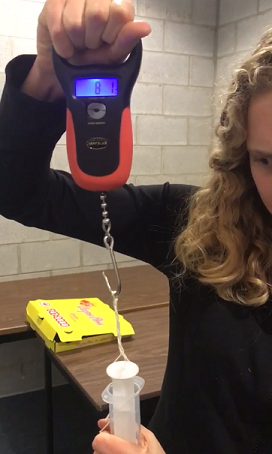
\includegraphics[width=50mm]{MeasuringSlidingFriction.png}
  \captionsetup{justification=centering}
  \caption{Measuring sliding friction force.}
  \label{fig:2}
\end{figure}


\section{Discussion}
\underline{Measuring properties of the syringe}

The needle inner diameter is taken from the manufacturer's website. There is likely tolerance on the diameter, which could contribute to the overall deviation between the theoretical and measured values. However, the effect is small as the ratio between the inner diameter of the needle and the syringe still remains on the same order of magnitude and takes on approximately the same value with numbers of significant digits present in Equation \ref{eq:1}.

\noindent\underline{Measuring height}

The percent errors between the measured heights and the theoretical heights vary significantly between the three $\frac{dh}{dt}$ collected in the experiment as presented in Table 2. The error can be as low as 7.71\% to as high as 69.4\%. A general trend seen in both measured and theoretical values is that as the plunger velocity increases, the corresponding calculated and measured height  increases. A graphic representation is shown below in Figure \ref{fig:3}. Based on the figure, the data seems to suggest a parabolic relationship between the height of the fluid and the plunger velocity as shown by Equation \ref{eq:1-3} shown in the Section 1. However, insufficient data was collected to confirm this relationship with the experimental values.

\begin{figure}[h!]
\centering
  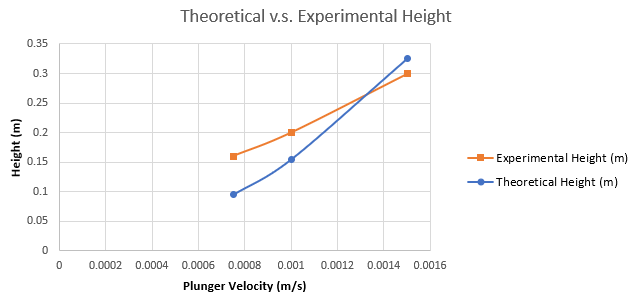
\includegraphics[width=150mm]{graph.png}
  \captionsetup{justification=centering}
  \caption{Theoretical and Experimental Heights in Different Plunger Velocity}
  \label{fig:3}
\end{figure}

The deviation between the two is mainly due to challenges encountered during data collection. The two main challenges faced were: it was very difficult to push down the syringe at a constant velocity and it was difficult to track the highest point of the jet stream from the video. Various attempts were made to improve the latter condition, including observing the shadow instead of looking at the transparent liquid and dying the water blue. However, these efforts were still futile, producing inaccurate readings of the measured values. In terms of the first challenge aforementioned, the resistance that had to be overcome by the experimenter to push the fluid through a needle with a diameter of 0.838 mm was tremendous. Often times the height of the jet stream was not maintained due to the difficulty in maintaining a constant velocity, as it requires pushing the syringe down at a constant force, which ultimately resulted in the error in the height of the jet stream measured. In addition, the experimenter who was pushing down the syringe had to keep track of the time in order to calculate the speed at which the piston was moving. These all contribute to error in the experimental values, resulting in the large percent error between the two.

\noindent\underline{Measuring sliding friction force}

As shown in Equation \ref{eq:10}, the force on the piston depends on the sliding friction force of the piston on the inside of the syringe body and the pressure force from the fluid inside the syringe. This pressure consists of two terms: one is the atmospheric pressure acting at the tip of the needle and the other is the capillary pressure at the air-water interface. Based on the relationship defining $F(v_{1})$ in \eqref{eq:11}, a higher plunger velocity would require a higher force exerted on the syringe, which makes sense intuitively. However, an interesting observation can be made based on the equation. It is shown that the theoretical force is mainly to overcoming $F_{s}$, the sliding friction of the piston, and pressure (atmospheric and capillary). A very small increase in force is seen when the plunger velocity increases. This is because the coefficient that the velocity is multiplied by is very small number (i.e. in order of magnitude of $10^{-6}$). In addition, realistic movement of the syringe falls in the range of mm/s, which is also a small number. 

This result reinforces the fact that it was hard to control the height of the jet stream as a small increase in force would lead to a big change in velocity. 

\section{Reflection}
Overall, the theoretical results agree with common sense in that, by increasing the force applied on the syringe, the plunger velocity increases which ultimately increase the height of the jet stream. However, real life modeling and application of fluid mechanics require much more thoughts and consideration when making assumptions. This experience was enlightening (and the struggle is real).


\setlength{\parindent}{1cm} 
\end{document}